\documentclass{extarticle}
\sloppy

%%%%%%%%%%%%%%%%%%%%%%%%%%%%%%%%%%%%%%%%%%%%%%%%%%%%%%%%%%%%%%%%%%%%%%
% PACKAGES            																						  %
%%%%%%%%%%%%%%%%%%%%%%%%%%%%%%%%%%%%%%%%%%%%%%%%%%%%%%%%%%%%%%%%%%%%%
\usepackage[10pt]{extsizes}
\usepackage{amsfonts}
\usepackage{amsthm}
\usepackage{amssymb}
\usepackage[shortlabels]{enumitem}
\usepackage{microtype} 
\usepackage{amsmath}
\usepackage{mathtools}
\usepackage{commath}
\usepackage[margin=1in]{geometry}
\usepackage{float}
\usepackage{cancel}
\usepackage{amsmath, amsfonts, amssymb}

%%%%%%%%%%%%%%%%%%%%%%%%%%%%%%%%%%%%%%%%%%%%%%%%%%%%%%%%%%%%%%%%%%%%%%
% PROBLEM ENVIRONMENT         																			           %
%%%%%%%%%%%%%%%%%%%%%%%%%%%%%%%%%%%%%%%%%%%%%%%%%%%%%%%%%%%%%%%%%%%%%
\usepackage{tcolorbox}
\tcbuselibrary{theorems, breakable, skins}
\newtcbtheorem{prob}% environment name
              {Problem}% Title text
  {enhanced, % tcolorbox styles
  attach boxed title to top left={xshift = 4mm, yshift=-2mm},
  colback=blue!5, colframe=black, colbacktitle=blue!3, coltitle=black,
  boxed title style={size=small,colframe=gray},
  fonttitle=\bfseries,
  separator sign none
  }%
  {} 
\newenvironment{problem}[1]{\begin{prob*}{#1}{}}{\end{prob*}}

%%%%%%%%%%%%%%%%%%%%%%%%%%%%%%%%%%%%%%%%%%%%%%%%%%%%%%%%%%%%%%%%%%%%%%
% THEOREMS/LEMMAS/ETC.         																			  %
%%%%%%%%%%%%%%%%%%%%%%%%%%%%%%%%%%%%%%%%%%%%%%%%%%%%%%%%%%%%%%%%%%%%%%
\newtheorem{thm}{Theorem}
\newtheorem*{thm-non}{Theorem}
\newtheorem{lemma}[thm]{Lemma}
\newtheorem{corollary}[thm]{Corollary}

%%%%%%%%%%%%%%%%%%%%%%%%%%%%%%%%%%%%%%%%%%%%%%%%%%%%%%%%%%%%%%%%%%%%%%
% MY COMMANDS   																						  %
%%%%%%%%%%%%%%%%%%%%%%%%%%%%%%%%%%%%%%%%%%%%%%%%%%%%%%%%%%%%%%%%%%%%%
\newcommand{\Z}{\mathbb{Z}}
\newcommand{\R}{\mathbb{R}}
\newcommand{\C}{\mathbb{C}}
\newcommand{\F}{\mathbb{F}}
\newcommand{\bigO}{\mathcal{O}}
\newcommand{\Real}{\mathcal{Re}}
\newcommand{\poly}{\mathcal{P}}
\newcommand{\mat}{\mathcal{M}}
\DeclareMathOperator{\Span}{span}
\newcommand{\Hom}{\mathcal{L}}
\DeclareMathOperator{\Null}{null}
\DeclareMathOperator{\Range}{range}
\newcommand{\defeq}{\vcentcolon=}
\newcommand{\restr}[1]{|_{#1}}


%%%%%%%%%%%%%%%%%%%%%%%%%%%%%%%%%%%%%%%%%%%%%%%%%%%%%%%%%%%%%%%%%%%%%%
% SECTION NUMBERING																				           %
%%%%%%%%%%%%%%%%%%%%%%%%%%%%%%%%%%%%%%%%%%%%%%%%%%%%%%%%%%%%%%%%%%%%%%
\renewcommand\thesection{\Alph{section}:}
\renewcommand\thesubsection{\Alph{section}.\arabic{subsection}}
\renewcommand\thesubsubsection{\Alph{section}.\arabic{subsection}.\arabic{subsubsection}}


%%%%%%%%%%%%%%%%%%%%%%%%%%%%%%%%%%%%%%%%%%%%%%%%%%%%%%%%%%%%%%%%%%%%%%
% DOCUMENT START              																			           %
%%%%%%%%%%%%%%%%%%%%%%%%%%%%%%%%%%%%%%%%%%%%%%%%%%%%%%%%%%%%%%%%%%%%%%
\title{\vspace{-2em}Chapter 8: The Philipps Curve (PC)}
\author{\emph{Summary}, by JF Viray}
\date{}

\begin{document}
\maketitle

\section{Deriving the PC}
Recall from the labor market, we have two relations:
\begin{align*}
    \text{ Wage-Setting (WS) Relation: } W &= P_t^e F\underset{(-}{(u_t}\underset{, +)}{, z)}  \\
    \text{Price-Setting (PS) Relation: } P_t &= (1+m) W 
\end{align*}

Since the price-setting relation expresses the price in terms of the wage, and we already know how the wage behaves, we can substitute the wage-setting relation into it. Rearranging then gives us:
$$P_t = P_t^e \cdot (1+m)  \cdot F(u, z)$$

Divide both sides by the price of last year ($P_{-1}$). It will also be convenient to suppose a specific form for the function $F$, so let $F(u_t, z) = 1 - \alpha u_t + z$ where $\alpha \in \mathbb{R}$ captures the strength of the effect of unemployment on the wage.
$$\frac{P_t}{P_{t-1}} = \frac{P_t^e}{P_{t-1}} \cdot (1+m) \cdot (1-\alpha u_t + z)$$

Recall from our definition of the inflation rate, $\pi = \frac{P_t - P_{t-1}}{P_{t-1}} = \frac{P_t}{P_{t-1}} - \frac{P_{t-1}}{P_{t-1}} = \frac{P_t}{P_{t-1}} - 1$. We can add 1 to both sides to have $\pi + 1 = \frac{P_t}{P_{t-1}}$. 
Similarly for the expected inflation, this equation holds: $\pi^e + 1 = \frac{P_t^e}{P_{t-1}}$. By substitution, we have:
$$(1+\pi) = (1+\pi^e) \cdot (1+m) \cdot (1-\alpha u_t + z)$$ 

We apply the natural log to both sides and have:
$$\ln (1+\pi) = \ln (1+\pi^e) + \ln (1+m) + \ln (1-\alpha u_t + z)$$
Use the approximation of $ln(1+x) \approx x$ when $x$ is small. Since we usually deal with numbers in the order of $10^{-2}$, we should be ok with assuming our numbers are small. Thus, we have:
$$\pi = \pi^e + m - \alpha u_t + z$$
This can further be cleaned to an equation to say that inflation today ($\pi$) is dependent on expected inflation ($\pi^e$), the markup ($m$), other factors in the labor market ($z$), and the unemployment rate ($u_t$). This is further shown with Figure 1 where as the unemployment rate ($u$) increases, the inflation rate ($\pi$) decreases.
$$\pi = \pi^e + (m+z) - \alpha u_t$$

\begin{figure}[H]
    \centering 
    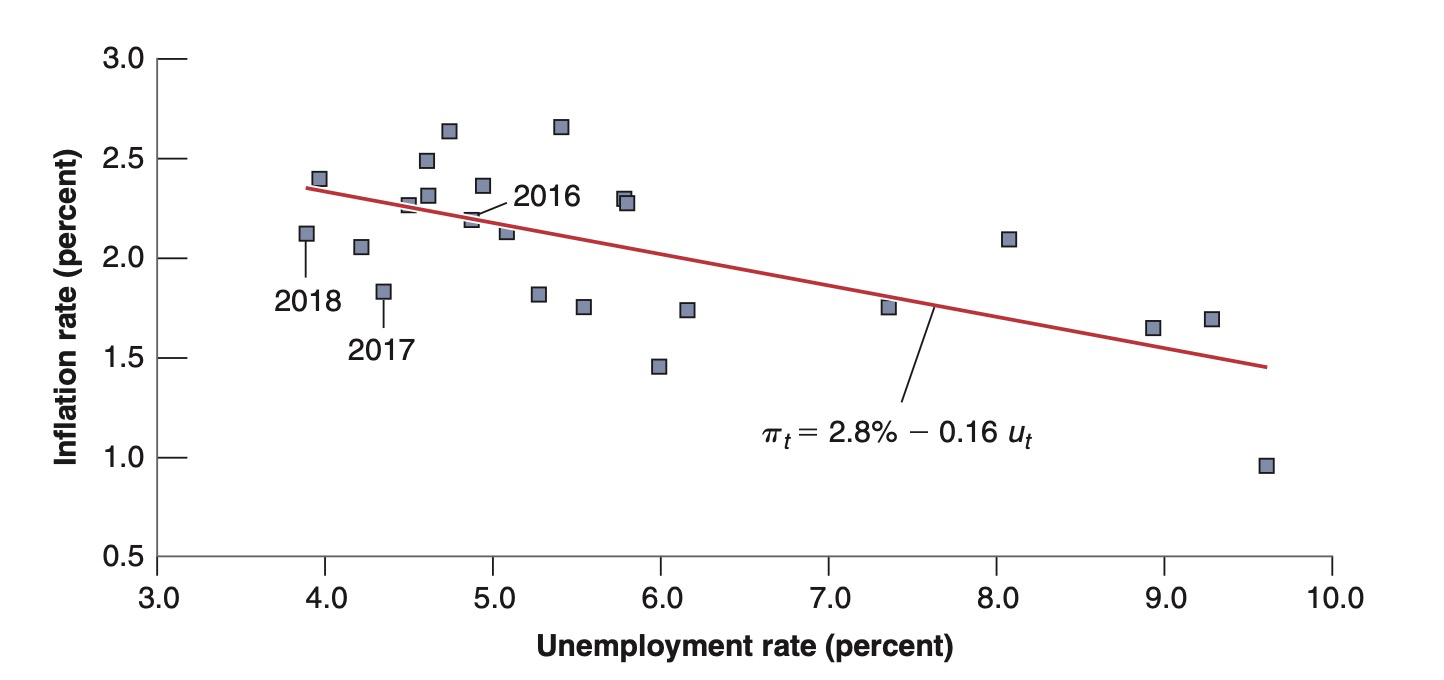
\includegraphics[width=0.5\linewidth]{PC.png} 
    \caption{Philipps Curve} 
    \label{fig:derivation} 
\end{figure}

Let's practice with this PC curve by playing with the variables. Recall that \textbf{everything ignites in the labor market}, so the chain of implications should be placed within the mechanisms of the wage-setting or price-setting relation. All we really did to get from the equilibrium in the labor market to the PC curve is (1) divide by the price level of the previous year ($P_{t-1}$), (2) rewrite all the things related to the price level in terms of the inflation rate, and (3) use the approximation of $\ln (1+x) \approx x$.
\begin{enumerate}
    \item What happens if expected inflation ($\pi^e$) increases?
    $$ \Delta P_e^+ \underbrace{\implies}_{\text{WS Relation}} \Delta W^+ \underbrace{\implies}_{\text{PS Relation}} \Delta P^+ \underbrace{\implies}_{\pi = \frac{P_t - P_{t-1}}{P_{t-1}}} \Delta \pi^+$$
    
    % \underbrace{\implies}_{\substack{\text{Equilibrium in} \\ \text{Labor Market}}} $$

    \item What happens if the unemployment increases?
    $$\Delta u_t^+ \underbrace{\implies}_{\text{WS Relation}} \Delta W^- \underbrace{\implies}_{\text{PS Relation}} \Delta P^- \underbrace{\implies}_{\pi = \frac{P_t - P_{t-1}}{P_{t-1}}} \Delta \pi^-$$
\end{enumerate}
\section{Accelerationist PC}
When expectations of the inflation rate is anchored to some stable historical average such as 2\%, we have $\pi^e = \overline{\pi}$. During the creation of the the original PC, expectatins were anchored, so we had:
$$\pi = \overline{\pi} + (m+z) - \alpha u_t$$
However, this did not last because wage-setters changed the way they formed their expectations about inflation. Expectations had been \textbf{de-anchored}, so wage-setters were expecting inflation to be of the previous year, NOT of the historical average. Let's model this as:
$$\pi_t^e = (1 - \theta) \overline{\pi} + \theta \pi_{t-1}$$
where $\theta$ is the strength of the belief that inflation yesterday will be inflation today. If $\theta = 0$, we had the anchored expectations where the expected inflation tomorrow is just the historical average. 
However, when $\theta = 1$, expected inflation today is just whatever was inflation yesterday, that is, $\pi^e = \pi_{t-1}$. 
In fact, what we instead have from the PC is NOT a formula for inflation, but it is rather a formula for the the CHANGE in inflation as shown below:



\begin{align*}
    \pi_t               &= \pi^e + (m+z) - \alpha u_t \\
    \implies \quad \quad \quad \quad \, \pi_t  &= \pi_{t-1} + (m+z) - \alpha u_t \\
    \implies \quad \pi_t - \pi_{t-1} &= (m+z) - \alpha u_t \\
    \implies \quad \quad \quad \; \; \, \Delta \pi        &= (m+z) - \alpha u_t
\end{align*}

This is what we call the accelerationist PC because inflation accelerates. It does not rise once and then drops back down to the historical average. Rather, this type of inflation can keep on growing.
\section{Natural Rate of Unemployment ($u_n$) and PC}
Recall from our discussion of the natural rate of unemployment ($u_n$), we assumed that expect and actual price level are the same ($P = P^e$). This would then mean that the expected inflation and actual inflation are also the same ($pi_t = \pi^e_t$). Thus, for the natural rate of unemployment ($u_n$), we have:
\begin{align*}
    \pi_t               &= \pi^e + (m+z) - \alpha u_n \\
    \implies \quad \pi_t - \pi_{e} &= (m+z) - \alpha u_n \\
    \implies \quad \quad \quad \; \; \, 0        &= (m+z) - \alpha u_n \\
    \implies \quad \quad \quad \, u_n &= \frac{m+z}{\alpha}
\end{align*}
We can then rewrite the original PC of $\pi = \pi^e + (m+z) - \alpha u_t$ in terms of the natural rate of unemployment. Notice:
\begin{align*}
    \pi_t               &= \pi^e_t + (m+z) - \alpha u_t \\
    \implies \quad \pi_t - \pi^e_t &= (m+z) - \alpha u_t \\
    \implies \quad \pi_t - \pi^e_t &= -\alpha(u_t - \frac{m+z}{\alpha}) \\
    \implies \quad \pi_t - \pi^e_t &= -\alpha(u_t - u_n)
\end{align*}
This equation is credibly important since it links the inflation rate, the expected inflation rate, and the deviation of the unemployment rate from the natural rate. This says the following:
\begin{enumerate}
    \item If unemployment is at the natural rate, then inflation will be equal to expected inflation. That is $u_t = u_n \implies \pi_t = \pi_t^e$
    \item If unemployment is BELOW the natural rate, then inflation will be higher than expected. That is $u_t < u_n \implies u_t - u_n < 0 \implies \pi_t - \pi_t^e > 0 \implies \pi_t > \pi_t^e$.
    \item If unemployment is ABOVE the natural rate, inflation will be lower than expected. That is $u_t > u_n \implies u_t - u_n > 0 \implies \pi_t - \pi_t^e < 0 \implies \pi_t < \pi_t^e$.
\end{enumerate}

\end{document}